% Karta eksploracji danych (M1). Kompilacja: latexmk -pdf M1_karta_eksploracji.tex  (w katalogu reports/)
% Liczby pochodzą z eda_numbers.tex i peaks_table.tex, generowanych przez: python -m pipeline.eda_twitter
\documentclass[10pt,a4paper]{article}
\usepackage[T1]{fontenc}
\usepackage[utf8]{inputenc}
\usepackage[polish]{babel}
\usepackage{lmodern}
\usepackage{microtype}
\usepackage[margin=1.7cm,top=1.5cm,bottom=1.6cm]{geometry}
\usepackage{booktabs,tabularx,array,graphicx,xcolor,enumitem}
\usepackage[hidelinks]{hyperref}
\setlist{nosep,leftmargin=*}
\setlength{\parskip}{3pt}\setlength{\parindent}{0pt}
\usepackage{titlesec}
\titleformat{\section}{\normalsize\bfseries}{\thesection.}{0.4em}{}
\titlespacing*{\section}{0pt}{6pt}{2pt}

% Wygenerowane przez python -m pipeline.eda_twitter. Nie edytować ręcznie.
\newcommand{\EdaNRows}{55\,035}
\newcommand{\EdaNRt}{35\,219}
\newcommand{\EdaNReply}{13\,773}
\newcommand{\EdaNOrig}{6\,043}
\newcommand{\EdaNAuthors}{18\,833}
\newcommand{\EdaNCascades}{20\,205}
\newcommand{\EdaNContents}{20\,188}
\newcommand{\EdaNDays}{312}
\newcommand{\EdaNBeforeEff}{39}
\newcommand{\EdaMedDaily}{131}
\newcommand{\EdaShareTrunc}{93,3\,\%}
\newcommand{\EdaShareBothOrig}{53,4\,\%}
\newcommand{\EdaShareScoreHigh}{93,2\,\%}
\newcommand{\EdaTopOnePctAuthors}{16,8\,\%}
\newcommand{\EdaTopTenSources}{22,6\,\%}
\newcommand{\EdaNPeaks}{8}
\newcommand{\EdaNPeaksRows}{6}
\newcommand{\EdaNPeaksOverlap}{1}
\newcommand{\EdaNRuDomain}{3}
\newcommand{\EdaNTme}{9}
\newcommand{\EdaNegShareRetweet}{33,1\,\%}
\newcommand{\EdaNegShareReply}{58,8\,\%}
\newcommand{\EdaPowerHalf}{46\,\%}
\newcommand{\EdaPowerHigh}{80\,\%}
\newcommand{\EdaCNeg}{55,6\,\%}
\newcommand{\EdaCPos}{7,2\,\%}
\newcommand{\EdaCAnti}{13,7\,\%}
\newcommand{\EdaCPro}{8,4\,\%}
\newcommand{\EdaCNegAnti}{9,4\,\%}
\newcommand{\EdaCPosPro}{1,4\,\%}
\newcommand{\EdaCNegGivenAnti}{68,3\,\%}
\newcommand{\EdaCNeuGivenAnti}{28,3\,\%}
\newcommand{\EdaCPosGivenPro}{17,1\,\%}
\newcommand{\EdaCNegGivenPro}{50,3\,\%}
\newcommand{\EdaCAntiGivenNeg}{16,9\,\%}
\newcommand{\EdaRNeg}{41,5\,\%}
\newcommand{\EdaRNegAnti}{7,0\,\%}
\newcommand{\EdaRPosPro}{1,9\,\%}
\newcommand{\EdaNWeeks}{44}
\newcommand{\EdaTrNegRho}{0{,}46}
\newcommand{\EdaTrNegP}{$p=0{,}002$}
\newcommand{\EdaTrAntiRho}{0{,}45}
\newcommand{\EdaTrAntiP}{$p=0{,}002$}
\newcommand{\EdaTrNegAntiRho}{0{,}48}
\newcommand{\EdaTrNegAntiP}{$p<0{,}001$}
\newcommand{\EdaTrProRho}{$-$0{,}64}
\newcommand{\EdaTrProP}{$p<0{,}001$}
\newcommand{\EdaTrPosRho}{$-$0{,}37}
\newcommand{\EdaTrPosP}{$p=0{,}013$}
\newcommand{\EdaElNegA}{52,7\,\%}
\newcommand{\EdaElNegB}{58,8\,\%}
\newcommand{\EdaElNegP}{$p<0{,}001$}
\newcommand{\EdaElAntiA}{11,0\,\%}
\newcommand{\EdaElAntiB}{14,0\,\%}
\newcommand{\EdaElAntiP}{$p<0{,}001$}
\newcommand{\EdaElNegAntiA}{7,3\,\%}
\newcommand{\EdaElNegAntiB}{10,0\,\%}
\newcommand{\EdaElNegAntiP}{$p<0{,}001$}
\newcommand{\EdaElProA}{9,6\,\%}
\newcommand{\EdaElProB}{6,8\,\%}
\newcommand{\EdaElProP}{$p<0{,}001$}
\newcommand{\EdaCorVolNegRho}{$-$0{,}26}
\newcommand{\EdaCorVolNegP}{$p<0{,}001$}
\newcommand{\EdaCorAntiProRho}{0{,}05}
\newcommand{\EdaCorAntiProP}{$p=0{,}423$}
\newcommand{\EdaCorNegAntiRho}{0{,}06}
\newcommand{\EdaCorNegAntiP}{$p=0{,}305$}
\newcommand{\EdaLikesPos}{97}
\newcommand{\EdaLikesNeg}{59}
\newcommand{\EdaLikesNeu}{27}
\newcommand{\EdaLikesPosNegP}{$p=0{,}004$}
\newcommand{\EdaLikesNegNeuP}{$p<0{,}001$}
\newcommand{\EdaRtAnti}{11}
\newcommand{\EdaRtNone}{7}
\newcommand{\EdaRtAntiP}{$p=0{,}154$}

\newcommand{\UZUP}[1]{\textcolor{red}{[#1]}}   % miejsca do uzupełnienia przez zespół
\newcommand{\repo}{\url{https://github.com/21bp37/AMC_lab/tree/ukraine-source}}

\begin{document}
\begin{center}
{\large\bfseries Karta eksploracji danych (M1)}\\[2pt]
{\bfseries Narracje o Ukraińcach w Polsce: czy prorosyjski Telegram wyprzedza polskojęzyczny X?}\\[1pt]
\small Zespół \UZUP{nazwa}\quad·\quad repozytorium: \repo\quad·\quad 19.10.2026
\end{center}

\section{Pytanie badawcze i hipotezy}
\textbf{Pytanie.} Czy w okresie 4.03--31.12.2022 wzrosty liczby treści o Ukraińcach w Polsce pojawiały się najpierw
w prorosyjskich kanałach Telegrama, a dopiero później w polskojęzycznym X/Twitterze, i z jakim opóźnieniem?

\textbf{H1 (kolejność).} Piki dziennej liczby postów o Ukraińcach w Polsce w kanałach prorosyjskich poprzedzają piki
w polskojęzycznym X: odsetek pików X, przed którymi w oknie 0--7 dni wystąpił pik prorosyjskiego Telegrama, jest wyższy
niż przy losowym położeniu pików, a dla kanałów proukraińskich (grupa kontrolna) efekt nie występuje albo jest słabszy.

\textbf{H2 (stałe opóźnienie).} Dla pików z narracjami antyukraińskimi opóźnienie X względem prorosyjskiego Telegrama
jest dodatnie i w przybliżeniu stałe: mediana 1--7 dni, rozstęp międzykwartylowy $\le 2$ dni.

\textbf{Zawężenia wobec sformułowań roboczych.} (a) „Polskie media” mierzymy jako polskojęzyczny X, bo tylko takie dane
mamy. (b) Mierzymy \emph{narracje antyukraińskie} (świadczenia, przestępczość, banderyzm itd.), a nie dezinformację:
ta wymaga weryfikacji prawdziwości twierdzenia, którą możemy wykonać najwyżej dla kilku największych pików.
(c) Zbieżność w czasie nie dowodzi przepływu treści (zob. sekcja~5).

\section{Źródła danych i zakres próby}
\begin{tabularx}{\linewidth}{@{}>{\raggedright\arraybackslash}p{2.3cm}X>{\raggedright\arraybackslash}p{3.4cm}@{}}
\toprule
Źródło & Zakres i pola & Stan \\
\midrule
X/Twitter, PL (zmienna zależna) & API v2 for Academic Research (dostęp sprzed zmian z II 2023), import do NodeXL;
posty po polsku z frazami „Ukraińcy” i „w Polsce”, 24.02--31.12.2022. \EdaNRows{} wierszy: \EdaNOrig{} oryginałów,
\EdaNReply{} odpowiedzi, \EdaNRt{} retweetów; \EdaNAuthors{} kont. Pola: czas, tekst, typ relacji, liczniki interakcji,
domeny, grupa NodeXL, etykieta i pewność sentymentu. & w repozytorium; przeanalizowane \\
Telegram (zmienna niezależna) & „Russian and Ukrainian War-related Telegram Channels Dataset”: 79,6\,mln postów z 4\,687
kanałów (2015--2024), sieć 18,2\,mln przekazań, etykieta strony (\emph{Pro-Russian / Pro-Ukrainian / Neutral}) dla
3\,074 kanałów z klastrowania Leidena. Pola posta: kanał, czas, tekst, wyświetlenia, przekazania. &
\textbf{jeszcze niewczytany}; filtr gotowy i przetestowany \\
\bottomrule
\end{tabularx}

\textbf{Jednostka analizy:} doba kalendarzowa (czas Europe/Warsaw) × platforma × strona kanału.
\textbf{Okno:} 4.03--31.12.2022 (303 dni); dni 24.02--3.03 wyłączone, bo zbiór X ma w nich tylko \EdaNBeforeEff{} wierszy.
\textbf{Próba Telegrama:} posty z okna, wspominające Ukrainę/Ukraińców \emph{i} Polskę/Polaków (wyrażenia RU/UK w
\texttt{pipeline/config.py}); kanały bez etykiety strony raportujemy osobno.

\section{Wyniki wstępnej eksploracji (X/Twitter)}
{\centering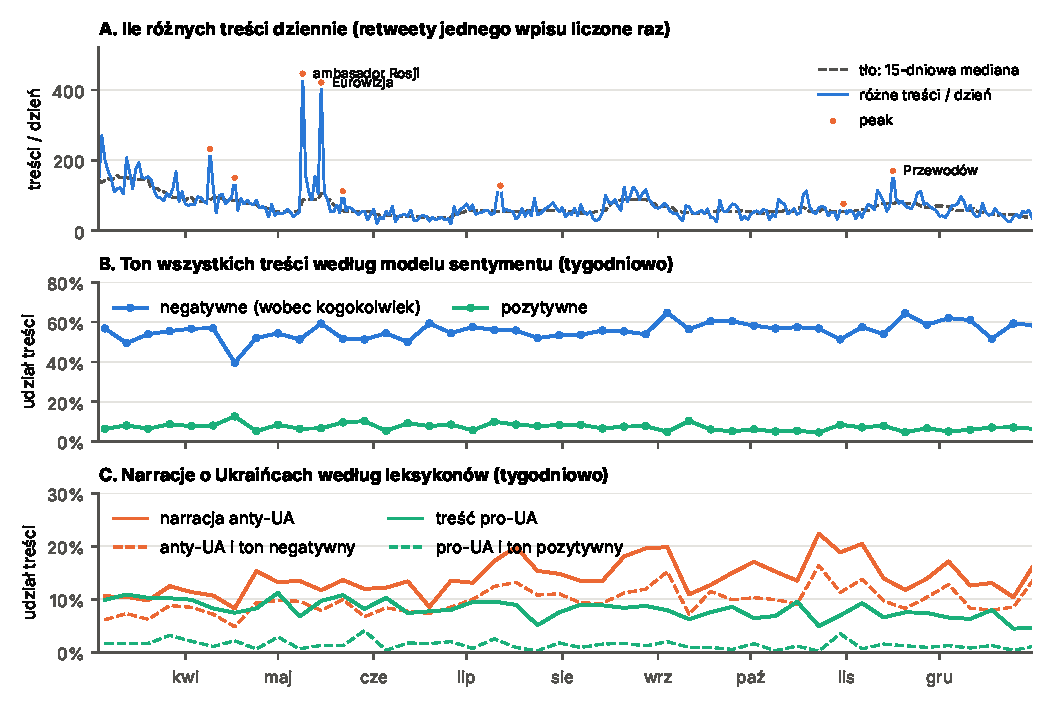
\includegraphics[width=0.92\linewidth]{figures/daily.pdf}\par}
{\footnotesize\textbf{Rys. 1.} Góra: liczba wierszy i liczba różnych treści (kaskad) na dzień, kropki: piki kaskad
($z>2{,}5$). Dół: kroczący 7-dniowy udział wierszy z sentymentem negatywnym i z trafieniem w leksykon narracji
antyukraińskich. Szare pole: okres niekompletny.\par}\vspace{2pt}
\begin{minipage}[t]{0.47\linewidth}\vspace{0pt}\footnotesize\setlength{\tabcolsep}{3.5pt}
% Wygenerowane przez python -m pipeline.eda_twitter.
\begin{tabular}{@{}lrrrl@{}}
\toprule
Dzień & Wpisy & Top konto & Negat. & Kontekst \\
\midrule
2022-05-15 & 1\,048 & 35\,\% & 54\,\% & Eurowizja \\
2022-05-09 & 877 & 17\,\% & 58\,\% & ambasador Rosji \\
2022-04-09 & 552 & 20\,\% & 43\,\% & -- \\
2022-05-22 & 367 & 22\,\% & 15\,\% & -- \\
2022-10-31 & 350 & 49\,\% & 62\,\% & -- \\
2022-11-16 & 291 & 14\,\% & 51\,\% & Przewodów \\
2022-04-17 & 289 & 27\,\% & 11\,\% & -- \\
2022-07-12 & 155 & 9\,\% & 48\,\% & -- \\
\bottomrule
\end{tabular}
\\[2pt]
\footnotesize Piki kaskad; „Top konto” = udział najczęściej retweetowanego konta w wierszach dnia.
\end{minipage}\hfill
\begin{minipage}[t]{0.5\linewidth}\vspace{0pt}
\begin{enumerate}[label=\textbf{E\arabic*.}]
\item \textbf{Zbiór jest niekompletny na starcie wojny:} mediana \EdaMedDaily{} wierszy/dzień, ale w 24.02--3.03 łącznie
\EdaNBeforeEff. Pierwsza fala narracji jest poza zasięgiem.
\item \textbf{Wolumen tworzą kaskady RT kilku kont:} 10 kont to \EdaTopTenSources{} retweetów, 1\,\% najaktywniejszych
kont daje \EdaTopOnePctAuthors{} wierszy. Piki wierszy i piki treści pokrywają się tylko w \EdaNPeaksOverlap{}
z \EdaNPeaksRows{} dni, dlatego miarą główną są kaskady.
\item \textbf{Mało pików:} \EdaNPeaks{} pików kaskad w 303 dniach; 3 z nich mają oczywisty polski bodziec (Eurowizja,
farba na ambasadorze Rosji, Przewodów).
\end{enumerate}
\end{minipage}
\begin{enumerate}[label=\textbf{E\arabic*.},start=4]
\item \textbf{Brak śladu źródła w samym X:} w linkach jest \EdaNRuDomain{} odwołań do rosyjskich domen państwowych
i \EdaNTme{} do Telegrama. Kierunku przepływu nie da się więc odczytać z X; potrzebny jest Telegram i porównanie w czasie.
\item \textbf{Sentyment nie mierzy narracji antyukraińskich:} etykieta \emph{negative} obejmuje \EdaShareNeg{} wierszy
(neutral \EdaShareNeu, positive \EdaSharePos), także krytykę Rosji i polskich polityków. Wśród trafień leksykonu negatywnych
jest \EdaLexNeg, poza nimi \EdaNoLexNeg; dzienna korelacja obu udziałów wynosi \EdaCorrNegLex. Model sentymentu jest
nieopisany, a \EdaShareScoreHigh{} etykiet ma pewność $>0{,}95$. Sentymentu nie używamy jako miary.
\item \textbf{Kryterium doboru nie zgadza się z opisem:} obie frazy dosłownie zawiera \EdaShareBothOrig{} oryginałów
i odpowiedzi (odmiana, synonimy); \EdaShareTrunc{} retweetów ma ucięty tekst. Leksykon narracji (v0.1, niezwalidowany)
trafia w \EdaShareLex{} wierszy. Negatywność jest wyższa w odpowiedziach (\EdaNegShareReply) niż w retweetach (\EdaNegShareRetweet).
\end{enumerate}

\section{Plan pomiaru zjawiska}
\begin{enumerate}[label=\arabic*.]
\item \textbf{Szeregi dzienne.} $Y_t$: liczba różnych kaskad w X o Ukraińcach w Polsce (H1) oraz z narracją antyukraińską
(H2). $X^{RU}_t$, $X^{UA}_t$: liczba postów z tematem w kanałach prorosyjskich i proukraińskich (kontrola); dla H2
również z narracją antyukraińską. Wariant ważony: suma wyświetleń.
\item \textbf{Narracje.} Leksykon PL v0.1 i odpowiednik RU/UK $\rightarrow$ klasyfikator (leksykon lub LLM z zapisanym
promptem). Walidacja: próba 2×300 postów (X, Telegram), warstwowana po trafieniu leksykonu i limitowana per konto/kanał,
kodowana przez 2 osoby; wymagane $\alpha$ Krippendorffa $\ge 0{,}667$; raportujemy P/R/F1 klasyfikatora
i korygujemy udziały estymatorem z próbą ekspercką (\texttt{tools/}).
\item \textbf{Piki.} Dzień, w którym $\log(1+x)$ przekracza 15-dniową kroczącą medianę o $z>2{,}5$ odpornych odchyleń
(1,4826·MAD) i jest maksimum w $\pm3$ dniach; czułość dla $z\in\{2;\,2{,}5;\,3\}$.
\item \textbf{Testy.} (i) Dopasowanie pików: odsetek pików $Y$ poprzedzonych pikiem $X$ w oknie 0--7 dni, rozkład zerowy
z 1000 kołowych przesunięć pików $X$. (ii) Korelacja krzyżowa przyrostów $\log(1+x)$ dla opóźnień $-14\ldots14$, test
permutacyjny. (iii) Granger w obu kierunkach. \textbf{H1 wspieramy}, gdy (i) daje $p<0{,}05$, (ii) ma maksimum przy
$k\in[1,7]$ z $r>0$, Granger $X^{RU}\!\to\!Y$ jest istotny, a $Y\!\to\!X^{RU}$ nie, oraz efekt dla $X^{RU}$ jest wyraźnie
silniejszy niż dla $X^{UA}$. \textbf{H2 wspieramy}, gdy dodatkowo mediana dopasowanych opóźnień leży w 1--7 dniach,
a IQR $\le 2$ dni (bootstrapowy przedział mediany).
\item \textbf{Ślad treści.} Dla 5 największych pików $Y$ ręcznie szukamy tego samego twierdzenia w Telegramie (tłumaczenie
RU$\to$PL) z datą wcześniejszą niż w X; to jedyny bezpośredni dowód przepływu.
\end{enumerate}

\section{Ograniczenia danych i możliwe źródła błędu}
\begin{itemize}
\item \textbf{Wspólny bodziec (najpoważniejsze):} obie platformy reagują na te same wydarzenia, a Telegram jest szybszy;
dodatnie opóźnienie może oznaczać szybkość platformy, nie przepływ. Ograniczamy to kontrolą proukraińską,
usunięciem dni z wydarzeniami z listy i śledzeniem treści (punkt~5).
\item \textbf{Moc testu:} w symulacji z 8 pikami i opóźnieniem 3 dni test (i) wykrywa efekt w \EdaPowerHalf{} prób, gdy
połowa pików X ma poprzednika na Telegramie, i w \EdaPowerHigh, gdy ma go 80\,\% (silne, 4-krotne piki; w danych
słabsze). \textbf{H2 przy ok. 8 pikach jest słabo oznaczalna}: IQR z kilku opóźnień jest niestabilny, więc H2
raportujemy opisowo, jeśli liczba dopasowanych pików będzie mniejsza niż 8.
\item \textbf{Dobór X:} nieznane dokładne zapytanie, luka 24.02--3.03, ucięte retweety, koncentracja na kilku kontach,
konta usunięte przed pobraniem są nieobecne. Grupy NodeXL to klastry sieci, nie etykiety ideologiczne.
\item \textbf{Telegram:} etykieta strony tylko dla 3\,074 z 4\,687 kanałów i na poziomie kanału (miary \texttt{antiukr},
\texttt{toxic} są zagregowane per kanał, nie per post); wyświetlenia z dnia pobrania, nie publikacji; temat w RU/UK
może być rzadki, co da zaszumione szeregi; wyrażenia filtra mogą łapać wzmianki niezwiązane z uchodźcami (np. o handlu z Polską).
\item \textbf{Pomiar narracji:} leksykon v0.1 bez walidacji; wspólny zestaw narracji dla PL i RU wymaga tłumaczenia
kategorii, nie słów. Strefy czasowe: oba źródła agregujemy do doby w czasie warszawskim.
\item \textbf{Etyka i licencje:} plik X z treściami i loginami jest w publicznym repozytorium; rekomendujemy zostawić
publicznie tylko ID postów (decyzja D1 w \texttt{CLEANUP.md}).
\end{itemize}

\section{Wykonalność do 5. zajęć}
\textbf{Gotowe:} pipeline X (wczytanie, kaskady, szeregi, piki, wykres, liczby do karty), filtr Telegrama w DuckDB
(strumieniowo, bez ładowania 79\,mln postów do pamięci), testy opóźnień i symulacja mocy; 23 testy na danych
syntetycznych, w tym odtworzenie znanego opóźnienia 3 dni i kalibracja testu przy braku efektu.\\[2pt]
\begin{tabularx}{\linewidth}{@{}lX@{}}
\toprule
Zajęcia 2 & Kopia zbioru Telegrama, uruchomienie filtra, liczności tematu per strona (\textbf{punkt krytyczny}). \\
Zajęcia 3 & Leksykon RU/UK, próba walidacyjna 2×300, kodowanie, $\alpha$; poprawki leksykonu. \\
Zajęcia 4 & Testy H1 z kontrolą, czułość progu i okna, śledzenie treści 5 pików. \\
Zajęcia 5 & H2 (lub opis, jeśli za mało pików), wyniki i ograniczenia do preprintu. \\
\bottomrule
\end{tabularx}\\[3pt]
\textbf{Wprost:} na samych danych z X hipotez nie da się zmierzyć (E4). Jeśli do 2. zajęć nie będziemy mieć Telegrama
albo dzienna liczba postów z tematem w kanałach prorosyjskich będzie bliska zera, H1 i H2 są nietestowalne i zawężamy
projekt do dynamiki narracji w X wokół wydarzeń. H1 na poziomie wolumenu tematu jest realna; H2 prawdopodobnie tylko
opisowo.

\section{Skład zespołu i role}
\begin{tabularx}{\linewidth}{@{}llX@{}}
\toprule
Osoba & Rola & Zakres \\
\midrule
\UZUP{imię i nazwisko} & Lead & pytanie, hipotezy, reguły decyzyjne, preprint \\
\UZUP{imię i nazwisko} & Inżynier danych & pozyskanie X i Telegrama, licencje, decyzje D1--D4 \\
\UZUP{imię i nazwisko} & Inżynier pipeline'u & \texttt{pipeline/}, testy, eksploracja, walidacja klasyfikatora \\
\UZUP{imię i nazwisko} & Analityk & leksykon narracji, kodowanie, testy H1/H2, interpretacja \\
\bottomrule
\end{tabularx}\\[2pt]
Repozytorium: \repo{}.\\ Wyniki odtwarza \texttt{python -m pipeline.eda\_twitter}; użycie AI opisuje
\texttt{09\_ujawnienie\_AI\_i\_wklad.md}.
\end{document}
